\documentclass{udpreport}
\title{Topología Física y Lógica de una red LAN}
\author{Integrantes: Thomas Muñoz, Ignacio Yanjari, Dagoberto Navarrete, Ignacio López.}
\date{Marzo de 2016}
\usepackage{graphicx}
\graphicspath{ {img/} }
\udpschool{Escuela de Informática y Telecomunicaciones}

\begin{document}
\maketitle
\tableofcontents % Despliega el índice
\chapter{Introducción}
En este laboratorio se buscó reconocer la composición de la red del laboratorio de Informática, identificando el hardware de red y los elementos que forman parte de ella, ya sean computadores, routers, switch, cables, etc. Se realizó también un diagrama de red, el cual especifica la información de los dispositivos que forman parte de esta (IP y MAC de cada uno)"agregar"(lo que escriba yo no lo tomen en cuenta si sienten que esta mal! :c  Se realizó también un diagrama de red, el cual especifica la información tanto de los pc´s(IP y MAC de cada uno ), la informacion de el switch y path.)
\chapter{Actividades}
\section{Identificación de elementos de red}
Para poder identificar el IP y MAC de cada computador, fue necesario abrir la terminal de cada Pc.
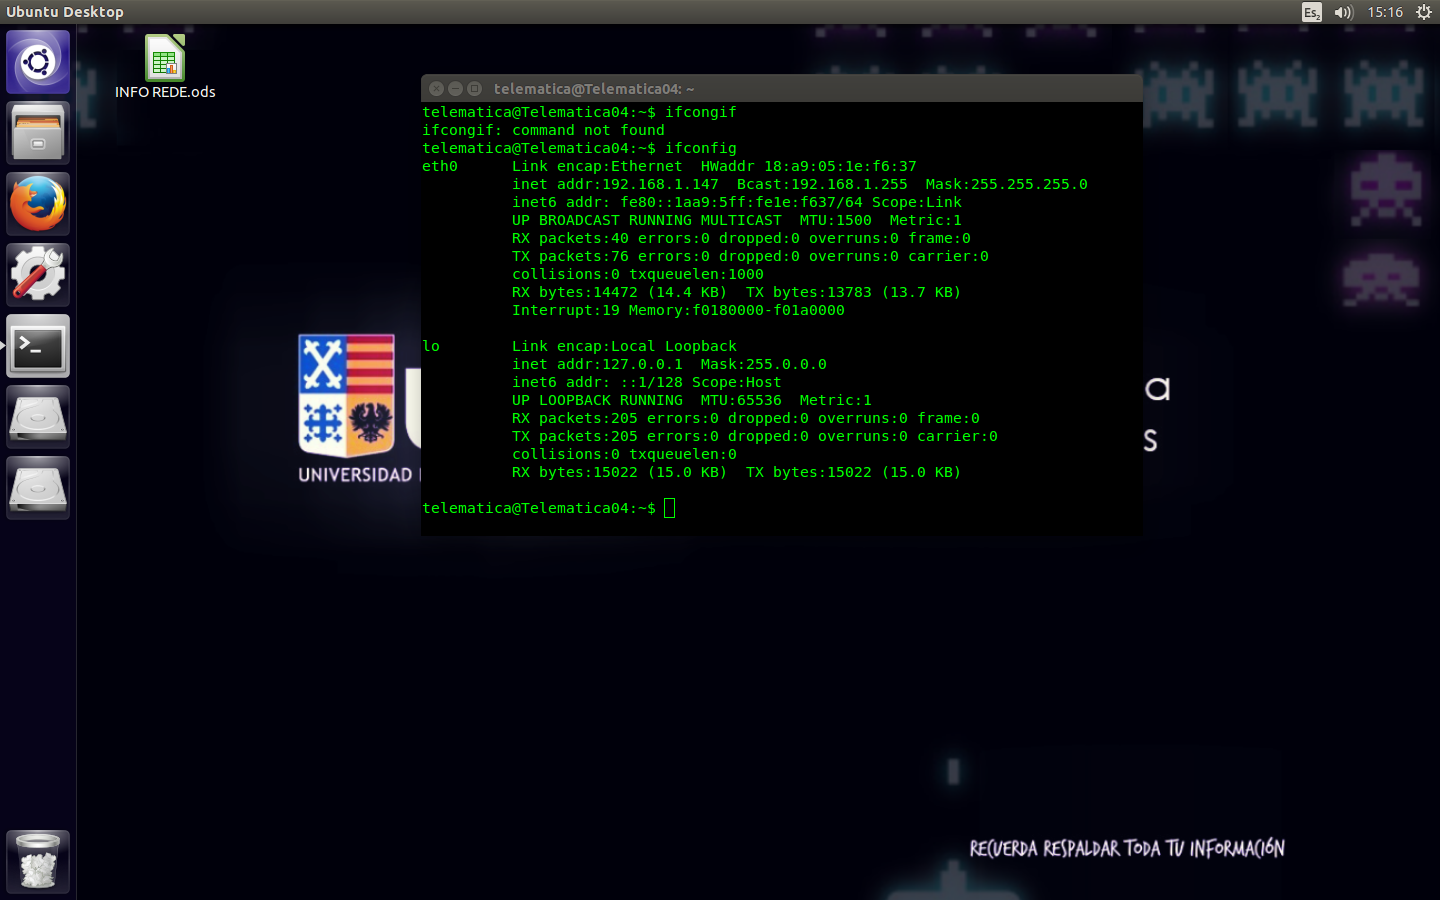
\includegraphics[witdth=\textwidth]{Terminal.png}
Por ejemplo ( imagen sacada de otro Pc) la MAC de el nuevo computador es MAC(Hwaddr denotado en el terminal) = 18:a9:05:1e:f6:37
la ip se denota como inet addr =192.168.1.147.Luego de ya obtener estos datos procedimos a observar el cable de red
para saber de que tipo es,para lograr esto es necesario simplemente ver el cubierto de el cable,al terminar , simplemente queda observar como se ubica el switch y  patch con los conectores,las caracteristicas a observar para luego analizar son en la forma en la que se conectan el patch con los equipos, al decir esto me refiero a la estructura que tiene, la cual puede ser estrella,arbol, hibrida,etc y los numeros en los cuales se insertaron cada conector(n° en el patch y switch). 
%nose si realmente colocar eso que escribieron abajo de este comentario ;C
El laboratorio cuenta con 18 computadores HP modelo EliteDesk 800 G1, conectados con cables UTP categoría 5e a un a un switch Cisco Catalyst 2960 el cual a su vez está conectado a un patch panel"revisar"(para luego ser conectador ordenadamente en el switch y ver un mejor orden al momento de ver alguna falla en algun dispositivo).
\section{Información de los dispositivos}
%Aca deberia ir el modelo de el path y el swtich tambien el modelo de los cables conectados uno a uno con el switch
\section{Diagrama de red}
\includegraphics[width=\textwidth]{diag.png}
%Texto
\chapter{Conclusión}
%Texto
\end{document}
